% 2009 年四川卷文科第 19 题：正方形 ABCD 与平面四边形 ABEF 所在平面互相垂直。
% 来源 PDF：普通高考/2009/2009四川文.pdf，SHA256 2bb14d3824466d9566238b20ec9270686c67d6e4f2af4186fd22b2a14e633ea7
% 原页：第 2 页（A3 三栏）第 1 栏上部，印刷页 560。
% 重绘依据：正方形按斜投影画成平行四边形 A 左下、B 右下、C 右上、D 左上；ABEF 所在平面竖直，
%   E 在 A 正上方、F 在 E 左侧；P 为 CD 中点、M 为 AE 中点，PM 细线；标注按各顶点外法向避让。
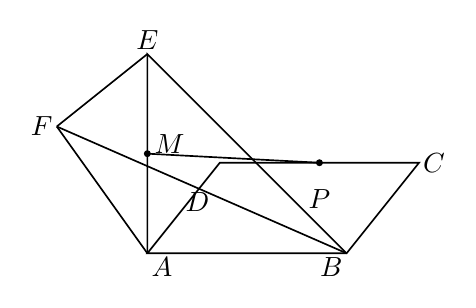
\begin{tikzpicture}[scale=1.15, semithick, every node/.style={inner sep=1.2pt}]
  \coordinate (A) at (0,0);
  \coordinate (B) at (2.2,0);
  \coordinate (C) at (3.0,1.0);
  \coordinate (D) at (0.8,1.0);
  \coordinate (E) at (0,2.2);
  \coordinate (F) at (-1.0,1.4);
  \coordinate (P) at (1.9,1.0);
  \coordinate (M) at (0,1.1);
  % 正方形
  \draw (A) -- (B) -- (C) -- (D) -- cycle;
  % 四边形 ABEF 与连线
  \draw (A) -- (E) -- (B);
  \draw (F) -- (A);
  \draw (F) -- (E);
  \draw (F) -- (B);
  % 中点与 PM
  \fill (P) circle (1.1pt);
  \fill (M) circle (1.1pt);
  \draw (P) -- (M);
  \node[anchor=north west] at (A) {$A$};
  \node[anchor=north east] at (B) {$B$};
  \node[anchor=west] at (C) {$C$};
  \node[anchor=north east] at ([xshift=-2pt,yshift=-8pt]D) {$D$};
  \node[anchor=south] at (E) {$E$};
  \node[anchor=east] at (F) {$F$};
  \node[anchor=north] at ([yshift=-7pt]P) {$P$};
  \node[anchor=west] at ([xshift=1pt,yshift=3pt]M) {$M$};
\end{tikzpicture}
